% Figure 2: Problem 2 - pod path broken while the node stays Ready
% Same drawing as in ppt/project2/slides.tex. Compile: pdflatex fig2_problem2_single_path.tex
\documentclass[border=4pt]{standalone}
\usepackage{amssymb}
\usepackage{tikz}
\usetikzlibrary{arrows.meta, positioning, fit, backgrounds, calc}
\renewcommand{\familydefault}{\sfdefault}
\tikzset{
  box/.style={draw, rounded corners, align=center, font=\scriptsize,
    minimum width=2.4cm, minimum height=0.6cm},
  arr/.style={-{Stealth[length=1.6mm]}, thick},
  biarr/.style={{Stealth[length=1.6mm]}-{Stealth[length=1.6mm]}, thick},
}
\begin{document}
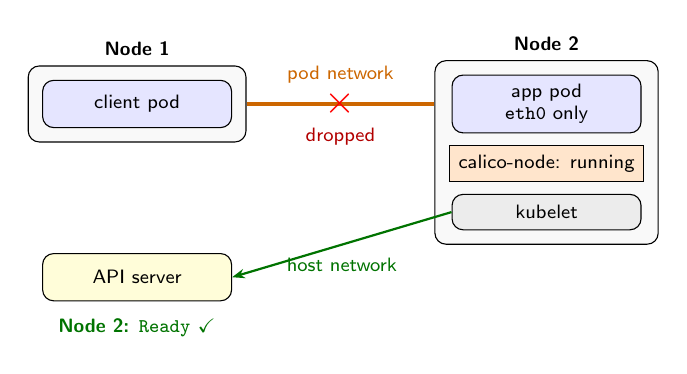
\begin{tikzpicture}[font=\scriptsize]
  % nodes
  \node[box, fill=blue!10] (cli) at (0,0) {client pod};
  \node[box, fill=blue!10] (app) at (5.2,0) {app pod\\\texttt{eth0} only};
  \node[box, fill=orange!20, below=0.15cm of app, rounded corners=0pt, minimum height=0.4cm] (cal) {calico-node: running};
  \node[box, fill=gray!15, below=0.15cm of cal, minimum height=0.45cm] (kl) {kubelet};
  \begin{scope}[on background layer]
    \node[draw, rounded corners, fill=gray!5, fit=(cli), inner sep=5pt,
      label={[font=\scriptsize\bfseries]north:Node 1}] (n1) {};
    \node[draw, rounded corners, fill=gray!5, fit=(app)(cal)(kl), inner sep=5pt,
      label={[font=\scriptsize\bfseries]north:Node 2}] (n2) {};
  \end{scope}
  % broken pod path
  \coordinate (mid) at ($(n1.east |- cli)!0.5!(n2.west |- app)$);
  \draw[very thick, orange!80!black] (n1.east |- cli) -- (n2.west |- app);
  \node[text=orange!80!black, above=4pt] at (mid) {pod network};
  \node[text=red, font=\Large\bfseries] at (mid) {$\times$};
  \node[text=red!70!black, below=5pt] at (mid) {dropped};
  % control path still fine
  \node[box, fill=yellow!15] (api) at (0,-2.2) {API server};
  \draw[thick, green!45!black, -{Stealth[length=1.6mm]}] (kl.west) -- (api.east)
    node[pos=0.5, below=1pt, align=center, text=green!45!black] {host network};
  \node[text=green!45!black, font=\scriptsize\bfseries, below=0.1cm of api] {Node 2: \texttt{Ready} \checkmark};
\end{tikzpicture}
\end{document}
